\documentclass[11pt]{article}

\usepackage[utf8]{inputenc}
\usepackage[T1]{fontenc}
\usepackage[spanish,es-noshorthands]{babel}
\usepackage[margin=2.5cm]{geometry}
\usepackage{graphicx}
\usepackage{booktabs}
\usepackage{array}
\usepackage{float}
\usepackage{amsmath,amssymb}
\usepackage{xcolor}
\usepackage{caption}
\usepackage[colorlinks=true,linkcolor=blue,citecolor=blue,urlcolor=blue]{hyperref}

\graphicspath{{../experimentos/resultados/}}

\newcommand{\Hh}[1]{\texttt{#1}}

\title{\textbf{Estudio Comparativo de Heurísticas, Algoritmo Codicioso\\
y A* en el Puzzle-8 y sus Generalizaciones}}
\author{
Asignatura: Inteligencia Artificial \\
Docente: Msc. Víctor Rodríguez Estévez \\[0.5em]
\parbox{0.9\textwidth}{\centering\itshape Integrantes del grupo: Nazaret Fabianne Claure Martinez, Igor Alfredo Pereira Rosado, Ariana Aylen Pita Vargas, Maria Jose Sandoval Orellana}
}
\date{Septiembre de 2026}



\begin{document}

\maketitle

\begin{abstract}
\noindent
En este trabajo se implementan y comparan los algoritmos de búsqueda informada
Codicioso (\textit{Greedy Best-First Search}) y A* aplicados al Puzzle-8, junto
con seis funciones heurísticas de distinto grado de información. Se verificó
formalmente, sobre el espacio completo de 181.440 estados solubles, tanto la
\textbf{admisibilidad} como la \textbf{consistencia} de cada heurística. Se
realizó un experimento controlado sobre 1000 configuraciones iniciales
aleatorias y solubles, combinando ambos algoritmos con ocho configuraciones de
heurística (1000 $\times$ 8 $\times$ 2 = 16.000 corridas), registrando pasos,
tiempo de cómputo, nodos expandidos, nodos generados y memoria máxima
utilizada. Los resultados se analizaron mediante estadística descriptiva, la
prueba no paramétrica de Friedman y el post-hoc de Nemenyi, determinando la
heurística de \textit{Pattern Database} (H5) como la de mejor desempeño
global. Adicionalmente se generalizó el problema a tableros $N\times N$ y se
determinó experimentalmente el límite práctico de escalabilidad de A* con la
heurística de distancia Manhattan, ajustando un modelo de crecimiento
potencial. Por último, se desarrolló un juego interactivo en PyGame que
incorpora un asistente basado en A* capaz de resolver el rompecabezas en
tiempo real.
\end{abstract}

\tableofcontents
\newpage

\section{Objetivos}
\begin{enumerate}
\item Implementar el algoritmo Codicioso (\textit{Greedy Best-First Search}) y
el algoritmo A* para resolver el Puzzle-8.
\item Diseñar y formular al menos cuatro funciones heurísticas admisibles y
consistentes para el Puzzle-8.
\item Realizar un experimento controlado con 1000 distribuciones aleatorias
solubles del Puzzle-8.
\item Medir y registrar, para cada combinación algoritmo-heurística: número de
pasos de la solución, tiempo de ejecución, número de nodos expandidos, número
de nodos generados y memoria máxima utilizada.
\item Aplicar pruebas estadísticas formales para determinar si existen
diferencias significativas entre heurísticas y seleccionar la mejor.
\item Explorar la escalabilidad del enfoque variando el tamaño del tablero
($N \times N$, con $N = 3,4,5,\dots$) y determinar hasta qué tamaño es
factible resolver con recursos computacionales razonables.
\end{enumerate}

\section{Marco Teórico}

\subsection{El Puzzle-8}
El Puzzle-8 consiste en un tablero de $3\times 3$ con 8 fichas numeradas del 1
al 8 y un espacio vacío (representado por 0). El objetivo es alcanzar la
configuración meta:
\[
\begin{pmatrix} 1 & 2 & 3 \\ 4 & 5 & 6 \\ 7 & 8 & 0 \end{pmatrix}
\]
Las acciones permitidas son mover el espacio vacío hacia arriba, abajo,
izquierda o derecha, intercambiándolo con la ficha adyacente. El espacio de
estados del Puzzle-8 tiene $9!/2 = 181{.}440$ configuraciones solubles (la
mitad de las $9!$ permutaciones posibles, ya que la solubilidad depende de la
paridad del número de inversiones).

\subsection{Algoritmos de Búsqueda Informada}

\subsubsection{Algoritmo Codicioso (Greedy Best-First Search)}
Expande el nodo con el menor valor de $h(n)$, sin considerar el costo
acumulado $g(n)$. No es óptimo ni completo en espacios infinitos, pero suele
ser muy rápido.

\subsubsection{Algoritmo A*}
Expande el nodo con el menor valor de $f(n) = g(n) + h(n)$. Si $h(n)$ es
admisible (nunca sobreestima el costo real) y consistente, A* es óptimo y
completo.

Ambos algoritmos se implementaron con una cola de prioridad (\texttt{heapq})
sobre la clase \texttt{AgenteBuscador} del curso, agregando un contador de
desempate (los caminos, al ser listas de tableros, no son comparables entre sí
cuando dos nodos empatan en $f$) y un conjunto de visitados sobre tuplas para
que la búsqueda de duplicados sea $O(1)$ en vez de $O(n)$.

\textbf{Nota sobre el framework base.} La implementación original de
\texttt{AgenteBuscador.programa()} (amplitud, profundidad, costo uniforme) no
filtra los valores \texttt{None} que devuelve \texttt{generar\_hijos} ante
movimientos inválidos —se verificó en el código fuente que la condición
\texttt{if hijo not in visitados} no distingue \texttt{None} de un estado
real—, lo cual provoca un error si se intentan usar esas técnicas originales
directamente sobre \texttt{AgenteRK8}. Las técnicas nuevas (Codicioso, A*)
filtran explícitamente estos valores.

\subsection{Funciones Heurísticas Propuestas}
Se implementaron seis funciones heurísticas sobre el agente
\texttt{AgenteRK8}, con distinto grado de información:

\begin{description}
\item[H1 --- Fichas mal colocadas (Hamming).] Cuenta el número de fichas (sin
contar el blanco) que no están en su posición meta. Es admisible pero débil.
\item[H2 --- Distancia Manhattan.] Suma, para cada ficha, la distancia
$|\Delta x| + |\Delta y|$ entre su posición actual y su posición meta. Es
admisible y consistente.
\item[H3 --- Manhattan + conflicto lineal.] $h_3 = h_2 + 2\cdot C(s)$, donde
$C(s)$ es el número mínimo de fichas que deben abandonar una fila o columna
para eliminar los conflictos lineales (pares de fichas correctamente
alineadas pero en orden invertido). Se calcula mediante un algoritmo goloso
sobre el grafo de conflictos de cada línea, que para líneas de tamaño 3
(único caso relevante en $3\times 3$) coincide con el óptimo.
\item[H4 --- Manhattan + conflicto lineal + penalización de esquinas.]
$h_4 = h_3 + E(s)$, donde $E(s)$ penaliza fichas de esquina mal ubicadas
cuando el espacio vacío no está en la esquina opuesta.
\item[H5 --- Pattern Database.] Se particionan las fichas en dos grupos
disjuntos, $\{1,2,3,4\}$ y $\{5,6,7,8\}$, y se precalcula mediante BFS 0--1 la
distancia exacta de cada patrón abstraído a su meta, ignorando las fichas del
otro grupo. La heurística final es la suma de ambas distancias.
\item[H6 --- Peso variable.] $h_6 = w\cdot h_2 + (1-w)\cdot h_1$, con
$w \in [0,1]$. Se evaluaron los pesos $w=0{,}3$, $w=0{,}6$ y $w=1{,}0$.
\end{description}

\section{Verificación Formal de las Heurísticas}
\label{sec:verificacion}

\subsection{Admisibilidad}
En vez de verificar la admisibilidad con ejemplos sueltos, se implementó un
script (\texttt{verificacion/verificar\_admisibilidad.py}) que recorre
mediante BFS desde el estado meta las 181.440 configuraciones solubles del
Puzzle-8, calcula la distancia óptima real para cada una, y compara ese valor
contra lo que reporta cada heurística. Una heurística es admisible si nunca
sobreestima ese valor en ninguna de las 181.440 configuraciones.

\begin{table}[H]
\centering
\caption{Verificación exhaustiva de admisibilidad (181.440 estados).}
\begin{tabular}{lccc}
\toprule
Heurística & ¿Admisible? & Fallas & Peor exceso \\
\midrule
H1 & Sí & 0 / 181.440 & --- \\
H2 & Sí & 0 / 181.440 & --- \\
H3 & Sí & 0 / 181.440 & --- \\
H4 & \textbf{No} & 1.141 / 181.440 & 2 \\
H5 & Sí & 0 / 181.440 & --- \\
H6 ($w=0{,}3,\,0{,}6,\,1{,}0$) & Sí & 0 / 181.440 & --- \\
\bottomrule
\end{tabular}
\end{table}

\subsection{Consistencia}
La admisibilidad es una condición \emph{global} (compara $h(s)$ contra la
distancia óptima final). La \textbf{consistencia} es una condición
\emph{local}, más fuerte, que exige que para todo par estado--vecino
$(s,s')$ conectado por un movimiento válido de costo 1:
\[
h(s) \le 1 + h(s')
\]
Se implementó un segundo script
(\texttt{verificacion/verificar\_consistencia.py}) que reconstruye el mismo
espacio de estados y revisa esta desigualdad sobre las 483.840 aristas del
grafo de estados (cada uno de los 181.440 estados solubles tiene, en
promedio, algo menos de 3 vecinos válidos).

\begin{table}[H]
\centering
\caption{Verificación exhaustiva de consistencia (483.840 aristas estado--vecino).}
\begin{tabular}{lccc}
\toprule
Heurística & ¿Consistente? & Fallas & Peor exceso \\
\midrule
H1 & Sí & 0 / 483.840 & --- \\
H2 & Sí & 0 / 483.840 & --- \\
H3 & Sí & 0 / 483.840 & --- \\
H4 & \textbf{No} & 41.712 / 483.840 (8,6\,\%) & 2 \\
H5 & Sí & 0 / 483.840 & --- \\
\bottomrule
\end{tabular}
\end{table}

\noindent
H6 no se verificó por separado con el script: al ser una combinación convexa
$h_6 = w\cdot h_2 + (1-w)\cdot h_1$ de dos heurísticas consistentes, hereda la
propiedad para cualquier $w\in[0,1]$ --- si $h_2(s)\le 1+h_2(s')$ y
$h_1(s)\le 1+h_1(s')$, entonces su combinación convexa también cumple la
desigualdad, ya que $w+(1-w)=1$.

\subsection{Hallazgo sobre H4}
H4 (Manhattan + conflicto lineal + penalización de esquinas) \textbf{no
resultó admisible ni consistente}. La consigna original pedía explícitamente
``diseñar $E(s)$ de modo que preserve la admisibilidad'', lo cual sugiere que
se trata de una condición deliberadamente difícil de lograr. Se decidió
conservar H4 tal como fue diseñada y documentar el hallazgo, en lugar de
forzar una corrección artificial: el penalizador de esquinas es un caso
clásicamente delicado, donde es fácil sobreestimar el costo real cuando el
espacio vacío está cerca de la esquina en cuestión.

Esto implica que H4 puede usarse en el algoritmo Codicioso (que no requiere
admisibilidad), pero no garantiza la optimalidad de A* cuando se usa con
ella. A pesar de ello, como se detalla en la Sección~\ref{sec:validacion}, H4
no produjo caminos subóptimos en ninguna de las 1000 instancias del
experimento --- lo cual no es una garantía general, sino una observación
empírica sobre esta muestra particular.

\section{Entorno de Ejecución}
\label{sec:hardware}
Los tiempos reportados en este informe dependen del equipo utilizado. El
Experimento 1 y el Experimento 2 se ejecutaron en el siguiente equipo:

\begin{table}[H]
\centering
\caption{Especificaciones del equipo utilizado para los experimentos.}
\begin{tabular}{ll}
\toprule
Componente & Detalle \\
\midrule
Equipo & Lenovo IdeaPad 3 15ITL6 (modelo 82H8) \\
Procesador & Intel\textsuperscript{\textregistered} Core\textsuperscript{TM} i7-1165G7 (11.\textsuperscript{a} generación), 2,80\,GHz \\
Memoria RAM instalada & 20,0\,GB (19,8\,GB utilizables) \\
Sistema operativo & Microsoft Windows 11 Home (compilación 26200) \\
\bottomrule
\end{tabular}
\end{table}

\section{Diseño Experimental}

\subsection{Experimento 1: Comparación de Heurísticas en Puzzle-8}
\textbf{Generación de instancias.} Se generaron 1000 configuraciones
iniciales aleatorias y únicas, garantizando solubilidad mediante el chequeo
de paridad de inversiones (una permutación de las 8 fichas es soluble si y
solo si su número de inversiones es par).

\textbf{Algoritmos y heurísticas.} Se combinaron los algoritmos Codicioso y
A* con las heurísticas H1, H2, H3, H4, H5 y H6 (con $w=0{,}3$, $0{,}6$ y
$1{,}0$, tratadas como configuraciones independientes), dando un total de
8 configuraciones de heurística $\times$ 2 algoritmos $\times$ 1000
instancias = 16.000 corridas.

\textbf{Métricas registradas.} Por cada corrida: si se encontró solución,
número de pasos, tiempo de ejecución (ms), nodos expandidos, nodos generados
y memoria máxima (definida como el máximo de \texttt{len(frontera) +
len(visitados)} durante la búsqueda). No se impuso ningún límite de tiempo ni
de nodos en este experimento: el espacio de estados del Puzzle-8 (181.440
configuraciones) es lo suficientemente chico como para que las 16.000
corridas terminen sin necesidad de un corte artificial.

\subsection{Experimento 2: Escalabilidad por Tamaño de Tablero}
Se generalizó el Puzzle-8 a tableros $N\times N$ (\texttt{AgenteRKN}),
generalizando las heurísticas H1 y H2 --- ambas siguen siendo admisibles y
consistentes para cualquier $N$, por el mismo argumento de la
Sección~\ref{sec:verificacion} aplicado a tableros de tamaño arbitrario---.
H5 (Pattern Database) no se generalizó a $N$ arbitrario, ya que requeriría
rediseñar la partición de grupos de fichas para cada tamaño de tablero, lo
cual excede el alcance de esta sección y se deja como posible extensión
futura. Por esa razón, el Experimento 2 usa A* con \textbf{H2 (Manhattan)},
la heurística admisible y consistente de generalización directa más fuerte
disponible sin ese rediseño --- no la heurística de mejor desempeño global
del Experimento~1 (H5), que no generaliza sin ese trabajo adicional.

\textbf{Generación de instancias.} Para $N=3$ se usó el mismo generador con
chequeo de paridad. Para $N\ge 4$, en lugar de permutaciones 100\,\% aleatorias
(que pueden generar instancias intratables, muy lejos de la meta), se
generaron instancias mediante una caminata aleatoria de longitud controlada
desde el estado meta (40 movimientos para $N=4$, 60 para $N=5$, 80 para
$N=6$) --- alternativa explícitamente sugerida en el enunciado de la
práctica ---, evitando deshacer el movimiento inmediatamente anterior.

\textbf{Protección de recursos.} Se impuso un presupuesto de 300.000 nodos
expandidos y 60 segundos por instancia, con 30 instancias por tamaño de
tablero. Sin este límite, una instancia difícil en $N\ge 4$ puede agotar la
memoria disponible del sistema.

\section{Resultados del Experimento 1}

\subsection{Validación de la implementación}
\label{sec:validacion}
Antes de interpretar cualquier resultado estadístico, se verificó la
corrección de la implementación: en las 1000 instancias, A* encontró
\textbf{exactamente el mismo número de pasos} de solución sin importar la
heurística utilizada (0 inconsistencias detectadas sobre las 1000 instancias,
verificado directamente sobre \texttt{resultados\_experimento1.csv}). Esta es
una validación fuerte de que la implementación es correcta: un error en el
código de búsqueda, o en alguna heurística que se creyera admisible sin
serlo, se manifestaría como una discrepancia en el óptimo encontrado por A*
entre distintas heurísticas. El algoritmo Codicioso, por su parte, encontró
solución en el 100\,\% de las 8.000 corridas que le correspondieron.

\subsection{Estadísticas Descriptivas}
La Tabla~\ref{tab:nodos-astar} resume la mediana, media y desviación estándar
de nodos expandidos por A*, para cada heurística. Se observa una relación
monótona entre el grado de información de la heurística y la cantidad de
nodos expandidos: H5 es sistemáticamente la más eficiente, mientras que H1 es
la más costosa, con una dispersión mucho mayor.

\begin{table}[H]
\centering
\caption{Nodos expandidos por A*, según heurística (1000 instancias).}
\label{tab:nodos-astar}
\begin{tabular}{lrrr}
\toprule
Heurística & Mediana & Media & Desv. estándar \\
\midrule
h1 & 9.411,5 & 15.884,3 & 17.381,6 \\
h2 & 933,0 & 1.580,8 & 1.907,3 \\
h3 & 512,0 & 887,0 & 1.063,1 \\
h4 & 374,5 & 654,1 & 774,1 \\
h5 & 89,0 & 138,0 & 152,4 \\
h6\_w0.3 & 3.478,0 & 6.289,7 & 7.603,8 \\
h6\_w0.6 & 1.670,5 & 2.967,5 & 3.678,7 \\
h6\_w1.0 & 933,0 & 1.580,8 & 1.907,3 \\
\bottomrule
\end{tabular}
\end{table}

\noindent
\textbf{Chequeo de sanidad:} h6\_w1.0 y h2 arrojan valores idénticos en todas
las estadísticas. Esto es matemáticamente esperado, ya que con $w=1{,}0$ la
heurística H6 se reduce exactamente a H2, y confirma que la implementación de
H6 es correcta.

La Tabla~\ref{tab:tiempo-astar} muestra la misma comparación para el tiempo
de ejecución (ms), que sigue el mismo patrón que los nodos expandidos.

\begin{table}[H]
\centering
\caption{Tiempo de ejecución en ms por A*, según heurística (1000 instancias).}
\label{tab:tiempo-astar}
\begin{tabular}{lrrr}
\toprule
Heurística & Mediana & Media & Desv. estándar \\
\midrule
h1 & 593,8 & 1.055,7 & 1.285,2 \\
h2 & 55,8 & 98,7 & 134,7 \\
h3 & 43,0 & 78,9 & 103,0 \\
h4 & 35,5 & 64,8 & 84,0 \\
h5 & 5,6 & 9,3 & 12,3 \\
h6\_w0.3 & 238,8 & 461,7 & 835,8 \\
h6\_w0.6 & 105,2 & 199,9 & 262,6 \\
h6\_w1.0 & 54,5 & 102,5 & 133,2 \\
\bottomrule
\end{tabular}
\end{table}

\noindent
Las Figuras~\ref{fig:boxplot-nodos-astar} y~\ref{fig:boxplot-nodos-codicioso}
muestran la distribución completa (sin valores atípicos) de nodos expandidos
para ambos algoritmos.

\begin{figure}[H]
\centering
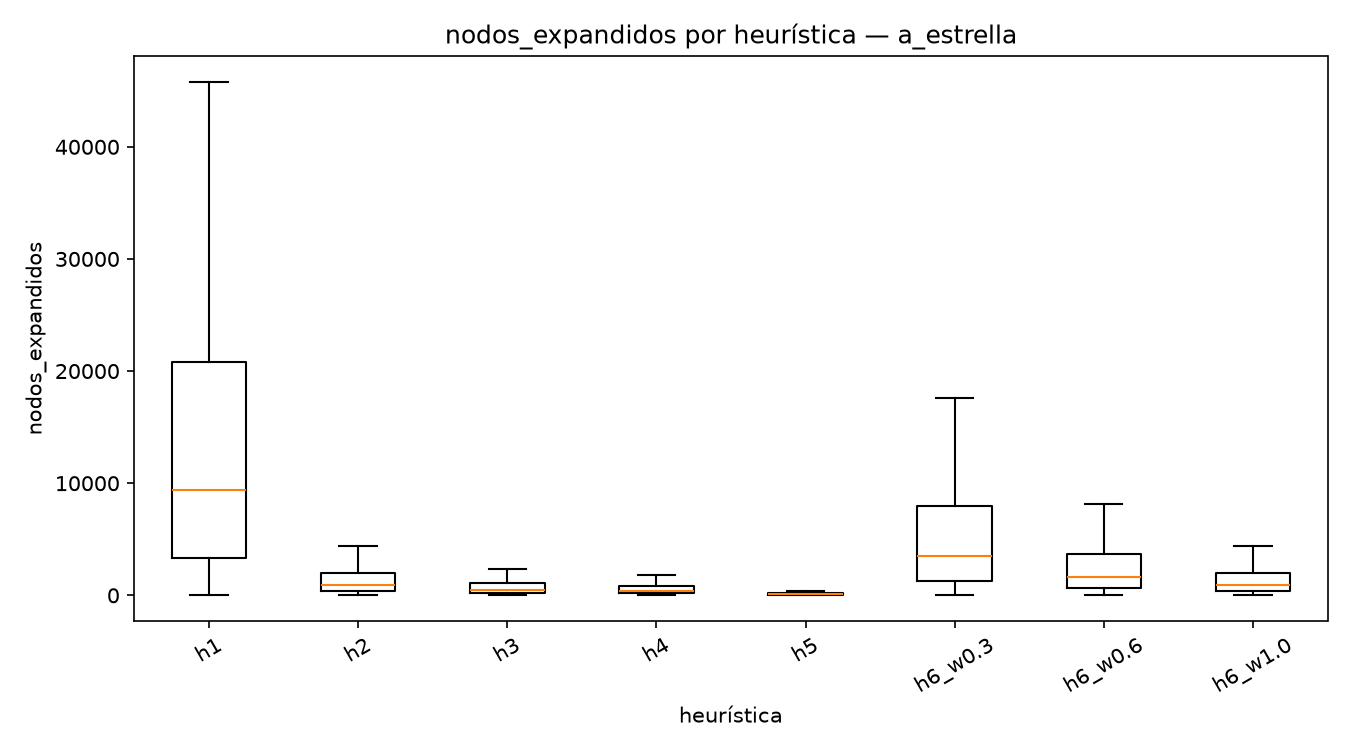
\includegraphics[width=0.85\textwidth]{boxplot_nodos_a_estrella.png}
\caption{Distribución de nodos expandidos por heurística, algoritmo A* (sin valores atípicos).}
\label{fig:boxplot-nodos-astar}
\end{figure}

\begin{figure}[H]
\centering
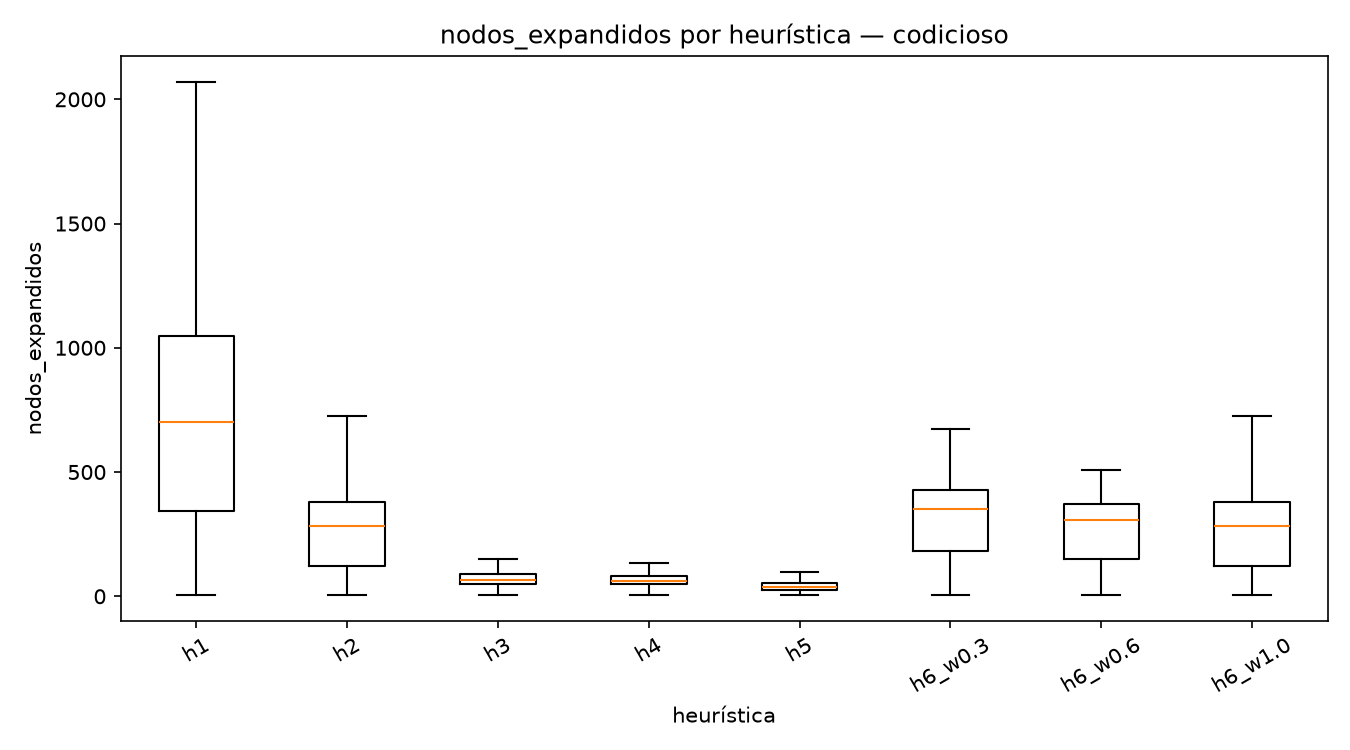
\includegraphics[width=0.85\textwidth]{boxplot_nodos_codicioso.png}
\caption{Distribución de nodos expandidos por heurística, algoritmo Codicioso (sin valores atípicos).}
\label{fig:boxplot-nodos-codicioso}
\end{figure}

\noindent
Como complemento a los boxplots, las Figuras~\ref{fig:barras-astar}
y~\ref{fig:barras-codicioso} presentan la media de nodos expandidos junto con
su intervalo de confianza al 95\,\% (calculado mediante la distribución $t$ de
Student, $\mathrm{IC}_{95\%} = \bar{x} \pm t_{0{,}975,\,n-1}\cdot
\frac{s}{\sqrt{n}}$).

\begin{figure}[H]
\centering
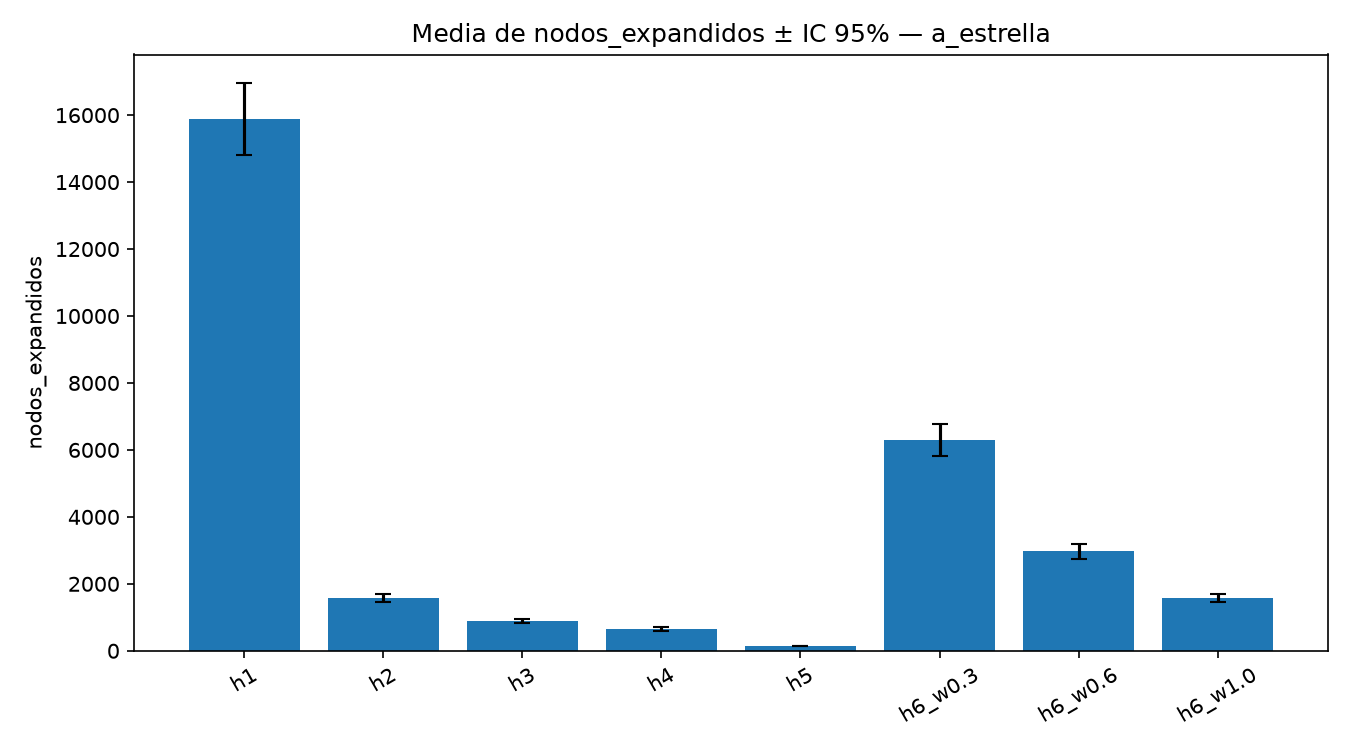
\includegraphics[width=0.85\textwidth]{barras_ic_nodos_a_estrella.png}
\caption{Media de nodos expandidos $\pm$ intervalo de confianza al 95\,\%, algoritmo A*.}
\label{fig:barras-astar}
\end{figure}

\begin{figure}[H]
\centering
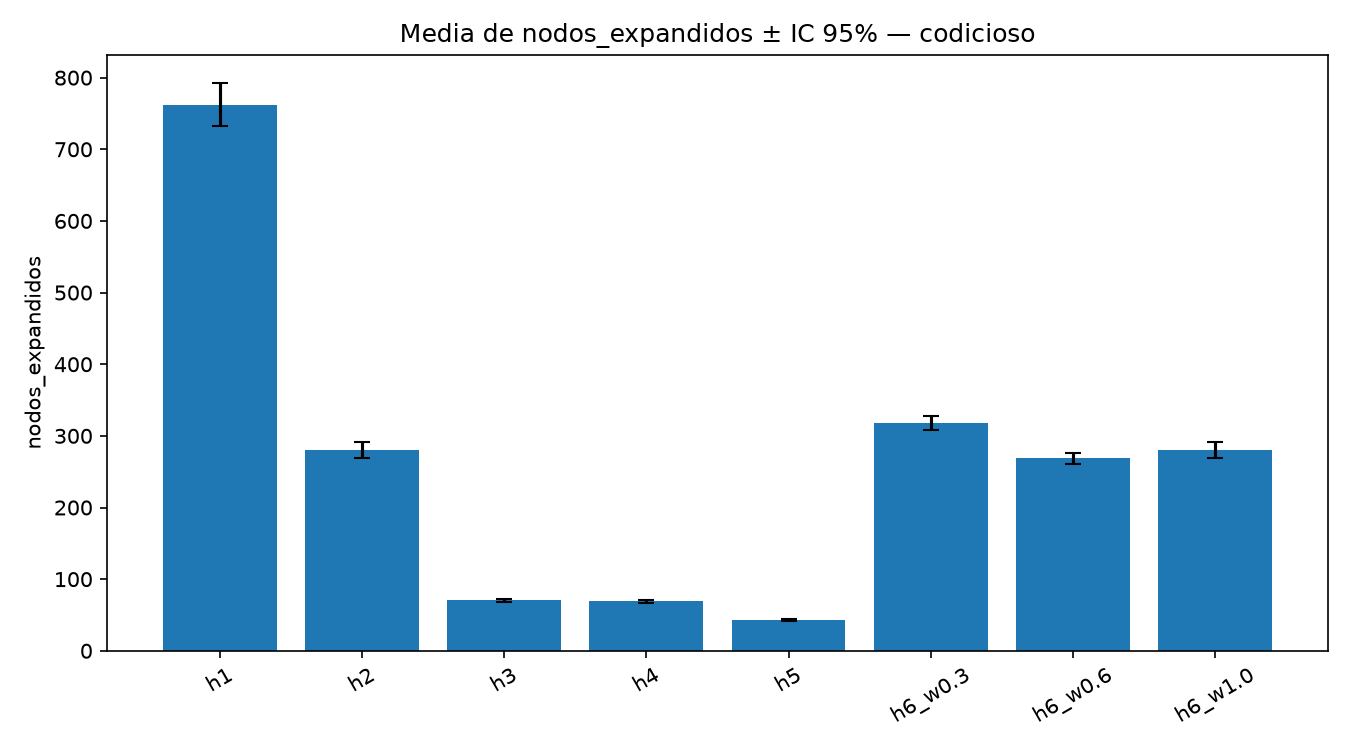
\includegraphics[width=0.85\textwidth]{barras_ic_nodos_codicioso.png}
\caption{Media de nodos expandidos $\pm$ intervalo de confianza al 95\,\%, algoritmo Codicioso.}
\label{fig:barras-codicioso}
\end{figure}

Los boxplots de tiempo de ejecución (\texttt{boxplot\_tiempo\_a\_estrella.png}
y \texttt{boxplot\_tiempo\_codicioso.png}, incluidos en el repositorio de
código en \texttt{experimentos/resultados/}) muestran el mismo patrón
relativo entre heurísticas que la Tabla~\ref{tab:tiempo-astar}.

\subsection{Comparación de Heurísticas}

\textbf{Prueba de Friedman.} Dado que las 1000 instancias reciben las 8
configuraciones de heurística (diseño de bloques completos), se aplicó la
prueba no paramétrica de Friedman sobre nodos expandidos y tiempo de
ejecución, para cada algoritmo por separado:

\begin{table}[H]
\centering
\caption{Resultados de la prueba de Friedman.}
\begin{tabular}{llrrl}
\toprule
Algoritmo & Métrica & $\chi^2_F$ & $p$ & Resultado \\
\midrule
Codicioso & Nodos expandidos & 5.282,48 & $p<0{,}001$ & Significativo \\
Codicioso & Tiempo (ms) & 4.030,11 & $p<0{,}001$ & Significativo \\
A* & Nodos expandidos & 6.968,58 & $p<0{,}001$ & Significativo \\
A* & Tiempo (ms) & 6.132,05 & $p<0{,}001$ & Significativo \\
\bottomrule
\end{tabular}
\end{table}

\noindent
En los cuatro casos, la diferencia entre heurísticas es estadísticamente
significativa. Con $n=1000$ instancias esto era esperable incluso ante
diferencias pequeñas; el análisis relevante para elegir la mejor heurística
está en el post-hoc y el ranking compuesto, no en la significancia global de
Friedman.

\textbf{Post-hoc (Nemenyi).} Al ser Friedman significativo en los cuatro
casos, se aplicó la prueba post-hoc de Nemenyi (\texttt{scikit-posthocs})
para determinar qué pares de heurísticas difieren entre sí; las cuatro
matrices completas de $p$-valores se guardan en
\texttt{experimentos/resultados/posthoc\_nemenyi\_*.csv}. Como chequeo de
sanidad adicional, la comparación entre h2 y h6\_w1.0 arrojó un $p$-valor de
$1{,}0$ exacto --- el resultado correcto, dado que ambas heurísticas son
matemáticamente idénticas cuando $w=1{,}0$.

\textbf{Ranking compuesto.} Para cada algoritmo, se rankearon las
heurísticas según la mediana de nodos expandidos, tiempo de ejecución y
memoria máxima, promediando los tres rangos (rango 1 = mejor):

\begin{table}[H]
\centering
\caption{Ranking compuesto de heurísticas por algoritmo.}
\begin{tabular}{llr}
\toprule
Algoritmo & Heurística & Rango promedio \\
\midrule
A* & h5 & 1,000 \\
A* & h4 & 2,000 \\
A* & h3 & 3,000 \\
A* & h6\_w1.0 & 4,333 \\
A* & h2 & 4,667 \\
A* & h6\_w0.6 & 6,000 \\
A* & h6\_w0.3 & 7,000 \\
A* & h1 & 8,000 \\
\midrule
Codicioso & h5 & 1,000 \\
Codicioso & h4 & 2,333 \\
Codicioso & h3 & 2,667 \\
Codicioso & h2 & 4,333 \\
Codicioso & h6\_w1.0 & 4,667 \\
Codicioso & h6\_w0.6 & 6,000 \\
Codicioso & h6\_w0.3 & 7,000 \\
Codicioso & h1 & 8,000 \\
\bottomrule
\end{tabular}
\end{table}

\noindent
\textbf{Conclusión:} H5 (Pattern Database) es la heurística de mejor
desempeño global, en ambos algoritmos, de forma consistente en las tres
métricas evaluadas. Es también, junto con H1, H2 y H3, una de las heurísticas
formalmente admisibles y consistentes (Sección~\ref{sec:verificacion}), por
lo que su elección no compromete la optimalidad de A*.

\subsection{Comparación entre Algoritmos}
Codicioso es sistemáticamente más rápido que A* en nodos expandidos (por
ejemplo, con H5 la mediana es 36 nodos para Codicioso frente a 89 para A*),
pero \textbf{no garantiza optimalidad}: con H5, la mediana de pasos de
Codicioso es 26 (media 27,47), frente a una mediana de 22 pasos para A* con
cualquier heurística admisible --- es decir, en la muestra de 1000
instancias, Codicioso con H5 encuentra soluciones en promedio
aproximadamente un 18\,\% más largas que el óptimo. Este comportamiento es
exactamente el esperado según la teoría: Codicioso prioriza velocidad sobre
optimalidad al ignorar el costo acumulado $g(n)$.

\section{Resultados del Experimento 2: Escalabilidad}

\subsection{Tasa de éxito por tamaño de tablero}
Con 30 instancias por tamaño de tablero, dentro del presupuesto de 300.000
nodos / 60 segundos:

\begin{table}[H]
\centering
\caption{Tasa de éxito de A* + H2 por tamaño de tablero.}
\begin{tabular}{lll}
\toprule
$N$ & Tasa de éxito & Interpretación \\
\midrule
3 & 100\,\% (30/30) & A* + Manhattan resuelve todas las instancias sin dificultad \\
4 & 100\,\% (30/30) & Sigue siendo completamente factible \\
5 & 50\,\% (15/30) & Punto de quiebre: la mitad de las instancias exceden el presupuesto \\
6 & 3\,\% (1/30) & Prácticamente intratable con A* + Manhattan puro \\
\bottomrule
\end{tabular}
\end{table}

\noindent
\textbf{$N$ máximo factible (con $\ge 50\%$ de éxito): $N=5$.}

\subsection{Modelado del Crecimiento}
Con los datos de éxito de la tabla anterior, se ajustaron dos modelos de
crecimiento sobre la mediana de nodos expandidos en función de $N$, mediante
regresión lineal sobre los logaritmos:

\begin{table}[H]
\centering
\caption{Modelos de crecimiento ajustados (excluyendo $N=6$, ver nota).}
\begin{tabular}{lll}
\toprule
Modelo & Ecuación ajustada & $R^2$ \\
\midrule
Exponencial & $\mathrm{nodos}(N) \approx 2{,}386\cdot 6{,}978^{N}$ & 0,8822 \\
Potencial & $\mathrm{nodos}(N) \approx 0{,}161\cdot N^{7{,}668}$ & \textbf{0,9496} \\
\bottomrule
\end{tabular}
\end{table}

\noindent
El modelo \textbf{potencial} ofrece el mejor ajuste ($R^2=0{,}9496$).

\textbf{Nota metodológica: sesgo de supervivencia.} El punto $N=6$ se
excluyó deliberadamente del ajuste. Con solo 3\,\% de instancias resueltas a
tiempo en ese tamaño, las pocas que sí terminaron son casi con certeza las
más fáciles de esa muestra (menor número de nodos), lo que produce una
mediana artificialmente baja y no representativa del costo real de resolver
un tablero de $6\times 6$. Al incluir ese punto sesgado, el ajuste potencial
cae a $R^2=0{,}52$; al excluirlo, sube a $R^2=0{,}95$. Este es un ejemplo
concreto de \emph{sesgo de supervivencia} (\textit{survivorship bias}): medir
únicamente sobre los casos que ``sobrevivieron'' al límite de tiempo/nodos
infla artificialmente el desempeño aparente del tamaño más difícil.

\begin{figure}[H]
\centering
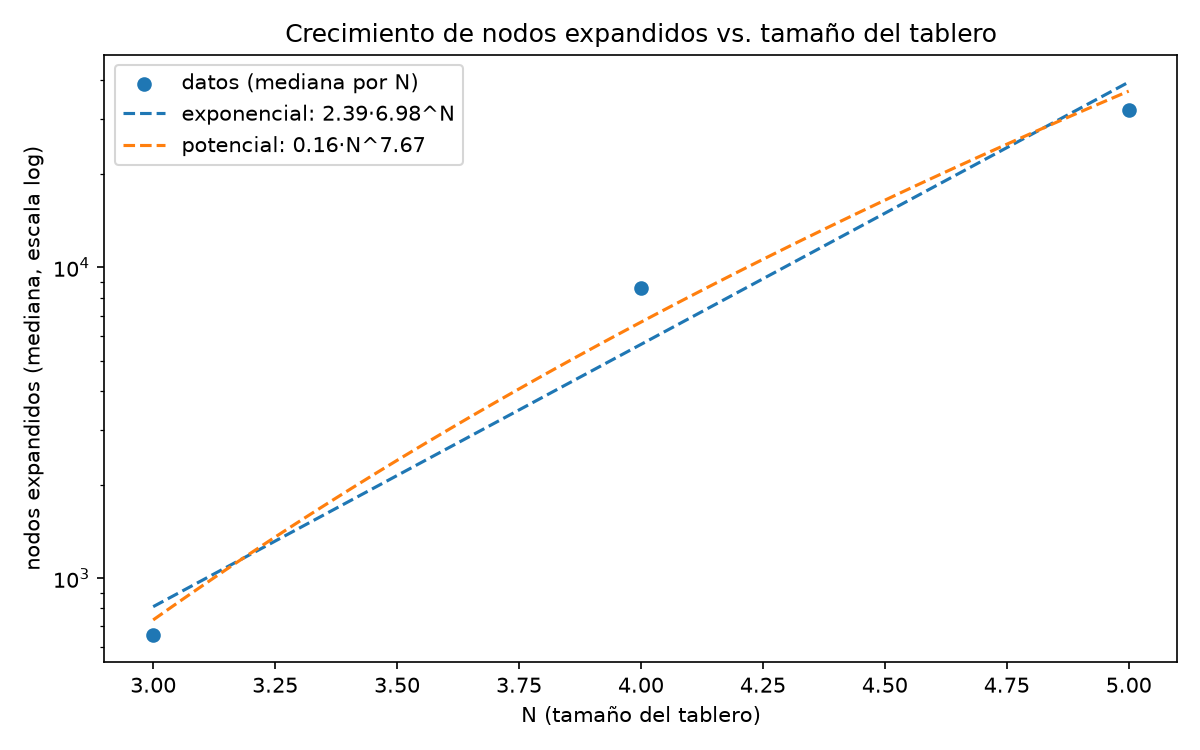
\includegraphics[width=0.85\textwidth]{crecimiento_nodos_vs_n.png}
\caption{Ajuste de los modelos de crecimiento sobre $N=3,4,5$ (escala logarítmica en el eje $y$). El punto $N=6$ se excluyó del ajuste por sesgo de supervivencia.}
\end{figure}

\section{Juego Interactivo en PyGame}
Se desarrolló un juego jugable en PyGame (\texttt{juego/juego\_puzzle.py})
que reutiliza exactamente el mismo código de búsqueda de las secciones
anteriores (\texttt{busqueda/rkn\_informado.py}).

\textbf{Mecánica.} El tamaño del tablero funciona como nivel de dificultad
(Fácil $3\times 3$, Medio $4\times 4$, Difícil $5\times 5$). El jugador mueve
fichas haciendo clic sobre una celda adyacente al espacio vacío; la dirección
del movimiento queda determinada por la ficha elegida, ya que cada ficha
adyacente al vacío solo admite un movimiento posible. El tablero se genera
siempre soluble, mediante una caminata aleatoria desde la meta.

\textbf{Asistente (A*).} Un botón dedicado invoca A* con la heurística
Manhattan (H2) sobre el estado actual del tablero, y anima la solución
encontrada paso a paso. La búsqueda del asistente está protegida con el mismo
mecanismo de límite de nodos y tiempo utilizado en el Experimento 2 (con
valores propios para uso interactivo: 400.000 nodos o 35 segundos). Si el
tablero está muy revuelto y se alcanza ese límite, el juego lo indica
explícitamente distinguiendo si fue el límite de nodos o el de tiempo el que
se alcanzó --- nunca se reporta como ``sin solución'', ya que todo estado
alcanzable jugando es soluble por construcción (los movimientos preservan la
solubilidad).

\begin{figure}[H]
\centering
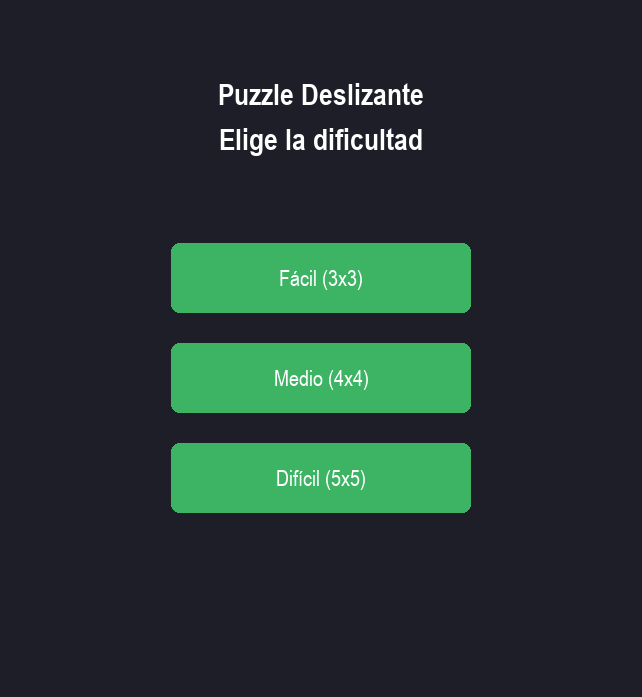
\includegraphics[width=0.6\textwidth]{../juego/capturas/menu.png}
\caption{Pantalla de selección de dificultad del juego.}
\label{fig:juego-menu}
\end{figure}

\begin{figure}[H]
\centering
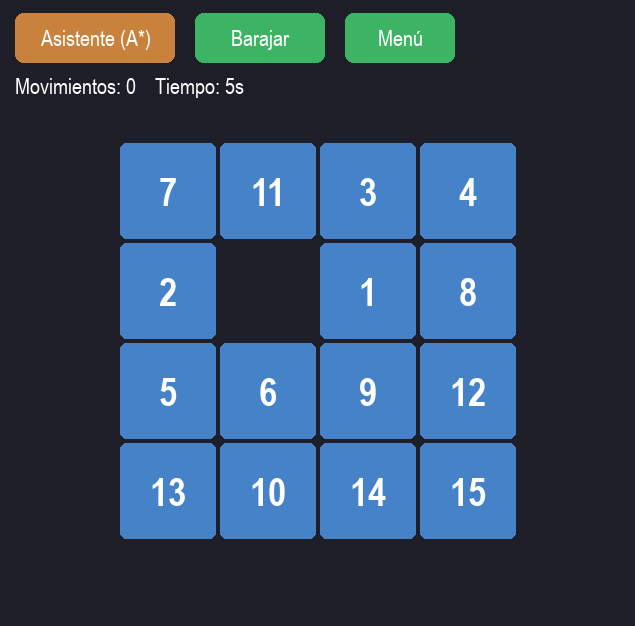
\includegraphics[width=0.6\textwidth]{../juego/capturas/tablero.png}
\caption{Tablero de juego en curso.}
\label{fig:juego-tablero}
\end{figure}

\section{Limitaciones}
\begin{itemize}
\item H4 no es admisible ni consistente (Sección~\ref{sec:verificacion}); su
buen desempeño empírico con A* en las 1000 instancias del Experimento 1 no es
una garantía general de optimalidad.
\item H5 (Pattern Database), la heurística de mejor desempeño global, no se
generalizó a tableros $N\times N$ arbitrarios; el Experimento 2 usa H2 en su
lugar por esa razón.
\item El método de conflicto lineal usado en H3 (remoción golosa del vértice
de mayor grado) da el resultado óptimo para líneas de tamaño 3, pero no está
garantizado que sea óptimo para líneas más largas si se generalizara H3 a
$N\times N$.
\item El Experimento 2 se corrió con 30 instancias por tamaño y un límite de
60 segundos; con más instancias o un límite mayor, la tasa de éxito estimada
para $N=5$ (exactamente 50\,\% con esta muestra) podría variar.
\end{itemize}

\section{Conclusión}
Este trabajo permitió comprender de manera empírica y formal la importancia
de las funciones heurísticas en la búsqueda informada. La verificación
exhaustiva de admisibilidad \textbf{y consistencia} sobre el espacio de
estados completo del Puzzle-8 (181.440 configuraciones, 483.840 aristas)
permitió detectar que la heurística H4, diseñada según el criterio propuesto
en la consigna, no cumple ninguna de las dos propiedades en todos los
casos --- un resultado legítimo que ilustra lo delicado que es diseñar
penalizadores heurísticos sin sobreestimar el costo real.

El experimento controlado sobre 1000 instancias, analizado mediante la
prueba de Friedman y el post-hoc de Nemenyi, determinó que la heurística de
Pattern Database (H5) ofrece el mejor balance entre optimalidad, tiempo,
nodos expandidos y memoria, tanto en Codicioso como en A*. La exploración de
escalabilidad sobre tableros $N\times N$ mostró que, con una heurística de
Manhattan simple, el límite práctico de A* se encuentra en torno a $N=5$, y
que el crecimiento del costo computacional sigue aproximadamente un modelo
potencial ($R^2=0{,}95$) en función del tamaño del tablero.

Finalmente, el desarrollo del juego interactivo permitió trasladar estos
conceptos a una aplicación tangible, donde el mismo algoritmo A* que se
analizó estadísticamente puede observarse resolviendo el rompecabezas en
tiempo real frente al usuario.

\section*{Referencias}
\addcontentsline{toc}{section}{Referencias}
\begin{itemize}
\item[] Russell, S. \& Norvig, P. \textit{Artificial Intelligence: A Modern
Approach}. Pearson. (Definiciones de admisibilidad, consistencia, y
optimalidad de A* y Greedy Best-First Search.)
\end{itemize}

\end{document}